\raggedright
\setlength{\parindent}{2em} %首行缩进
\newpage

\title{射影幾何自助餐} %標題
\author{Chen Xiang-Wei} %編輯這份講義的作者
\date{August 11, 2019}
\date{\today}%今天
\lfoot{Author:\theauthor}
\maketitle
\thispagestyle{fancy}
\raggedright
\rhead{模板}
\tableofcontents  % 生成目錄
%請在以下輸入內容

\setcounter{section}{-1}

\section{無窮遠炒麵線}
\pro
{\color[RGB]{0,255,200}對於}{\color{blue}複}\textbf{平}\textit{面}
~\\%空行
~\\%空行
上五點$z_{1}, z_{2}, z_{3},z_{4},z_{5}$,若\\
\[(z_{1},z_{2};z_{3},z_{4})=(z_{1},z_{2};z_{3},z_5)\]
則$z_{4}=z_{5}$\\


\pro 
$$
\frac{\cancel{n}}{si\bcancel{n} x}=\frac{1}{six}=\xcancel{\frac{1}{6}}
$$

\subsection[short]{特殊字}

\#
\$
\%
\{
\}
\~{}
\textbackslash
\^{}

\zhnumber{20120/20120}\\

\subsection{空行的方法}

\textbackslash vspace\{1cm\}
\vspace{1cm}

\~{}\textbackslash\textbackslash
~\\%空行

\subsection[short]{對齊}
\begin{alignat*}{4}
  &\text{組}&\text{別}:\ &\text{第14組}\\
  &\text{主寫}&\text{人}:\ &\text{我 }\\
  &\text{組}&\text{員}:\ &\text{你 }\\
       &&&\text{他 }\\
  &\text{日}&\text{期}:\ &\text{2023/09/10}\\
\end{alignat*}   


\subsection{表格}
\begin{tabular}[t]{|l|c|r|}
\hline%畫一條橫線
\diagbox{c}{r} & column2 & column3 \\
\hline%畫一條橫線
item1   & item2   & item3 \\
itemA   & itemB   & itemC \\
\hline
\end{tabular}

\subsubsection*{三線表}
\begin{tabular}{cccccc}
  \toprule
  序号 & 姓名 & 性别 & 年龄 & 身高/cm & 体重/kg \\
  \midrule
  1 & 张三 & M & 16 & 163 & 50 \\
  
  \cmidrule(lr){2-3}
  \cmidrule(lr){4-5}
  \cmidrule(lr){6-6}\morecmidrules\cmidrule(lr){6-6}

  2 & 王红 & F & 15 & 159 & 47 \\
  3 & 李二 & M & 17 & 165 & 52 \\
  \bottomrule
\end{tabular}





\begin{table}[ht]%這裡或頂部
  \begin{minipage}{.5\textwidth}
    \setlength{\abovecaptionskip}{0cm} % 调整caption间距
    \caption{第一次實驗吸光值}
      \label{tab:1}
      \begin{tabular}[t]{ccc}
        \toprule
        BSA (mg)&OD595nm&raw data\\
        \midrule
  0&0&0.122\\
  2&0.107&0.229\\
  4&0.12&0.242\\
  6&0.199&0.321\\
  8&0.244&0.366\\
  10&0.227&0.349\\
  5μl unknown&0.129&0.251\\
  10μl unknown&0.219&0.341\\
  
        \bottomrule
      
      \end{tabular}
  \end{minipage}
  \begin{minipage}{.5\textwidth}
  \caption{第二次實驗吸光值}
  \label{tab:2}
    \centering
      \begin{tabular}[t]{ccc}
        \toprule
        BSA (mg)&OD595nm&raw data\\
        \midrule
  0&0&0.119\\
  2&0.091&0.21\\
  4&0.102&0.221\\
  6&0.177&0.296\\
  8&0.229&0.348\\
  10&0.216&0.335\\
  5μl unknown&0.132&0.251\\
  10μl unknown&0.222&0.341\\
        \bottomrule
      
      \end{tabular}
  \end{minipage}
  \end{table}



  \begin{table}
    \centering
    \begin{tabular}{|c|c|c|c|}
      \hline
      \multirow{2}*{合并两行一列} & 二 & 三 & 四 \\
      \cline{2-4}
      ~ & 2 & 3 & 4 \\
      \hline
    \end{tabular}
  \end{table}
\subsection{方框}
\fbox{
  \parbox{\textwidth}{
想法:
容易發現$HA_{PH}C_{aH}C_{aP}, HB_{PH}C_{bH}C_{bP}, HC_{PH}C_{cH}C_{cP}$是平行四邊形,\\
欲構造共圓四點$UW_aW_bW_c$使$HA_{PH},HB_{PH},HC_{PH}$分別和$UW_a,UW_a,UW_a$\\
平行且長度比例相同即可證明命題\\

  }
}

\subsection{code}

\begin{lstlisting}
  import cv2
  import mediapipe as mp
  import numpy as np
  import statistics
  import math
\end{lstlisting}

\subsection{多欄位}
\begin{multicols}{2}
  \begin{enumerate}[label=(\roman*)]
  \item 取$P$為$\Delta ABC$垂心$H$
  \item {\color{blue}取$P$為$\Delta ABC$外心$O$}
  \item {\color[RGB]{0,255,200}取$Q$為$\Delta ABC$外心$O$}
  \item 取$P$為$\Delta ABC$外接圓上一點
  \item 取$P,Q$為同一點
  \item 取$Q$為$\Delta ABC$垂心$H$
  \item 當取$P$是定點時,$Q$滿足$H,A_3,B_3,C_3$四個共圓的軌跡不超過6次
  \end{enumerate}
\end{multicols}

\subsection{Footnote}
  我是原文\footnote{我是角標}



\newpage
\section{圖片}
\begin{figure}[H]
  \centering
  \begin{minipage}[b]{0.4\textwidth} %minipage寬
  \centering
  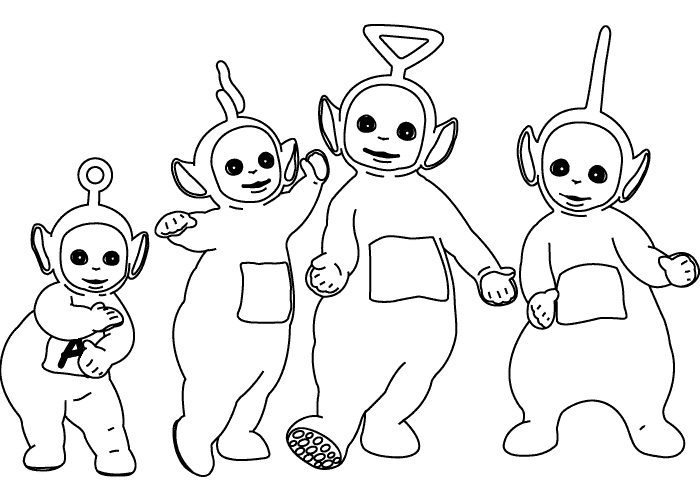
\includegraphics[width=1\textwidth]{a.png}
  \caption{正面照\upcite{dsd_tech2}}
  \label{fig:正面}
  \end{minipage}
  \begin{minipage}[b]{0.4\textwidth} %minipage宽
  \centering
  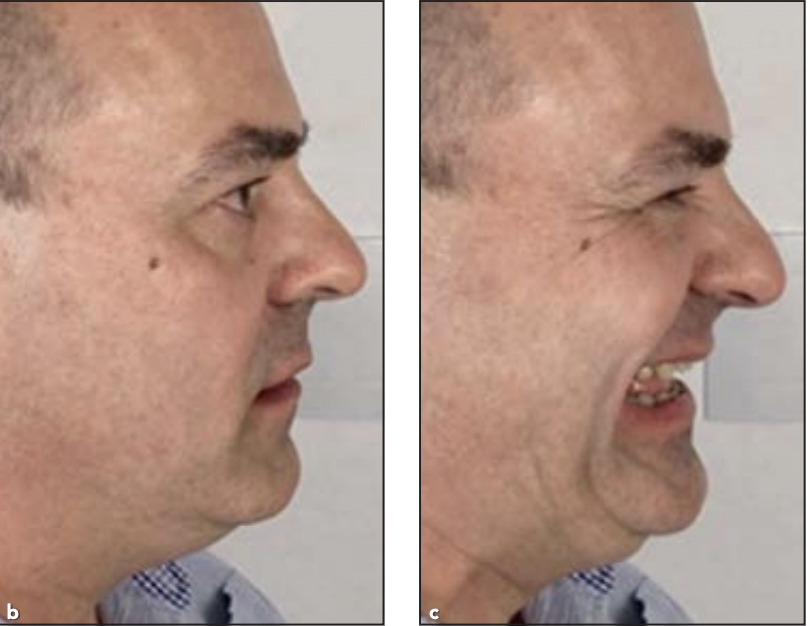
\includegraphics[width=1\textwidth]{paste_src/2023-02-07-20-50-39.png}
  \caption{側面照\upcite{dsd_tech2}}
  \label{fig:側面}
  \end{minipage}
  \end{figure}
  
\begin{figure}[H]%與文字並排
    \centering %圖片全居中
    %並排幾個圖就要開幾個minipage
    \begin{minipage}[b]{0.4\textwidth} %minipage寬
      \centering %图片局部居中
      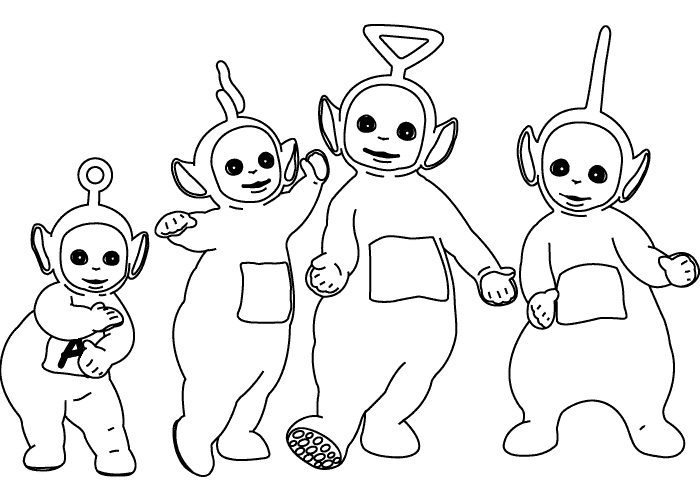
\includegraphics[width=0.8\textwidth]{a.png}
      \caption{最右邊是迪西}
      \label{fig:迪西}
    \end{minipage}
    \begin{minipage}[b]{0.4\textwidth} %minipage宽
      \centering %图片局部居中
      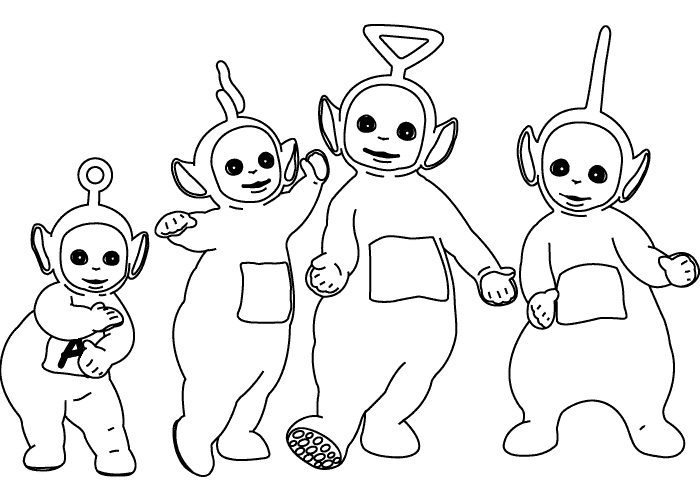
\includegraphics[width=0.8\textwidth]{a.png}
      \caption{再來是丁丁}
      \label{fig:丁丁}
    \end{minipage}
  \end{figure}
  所以
  丁丁是\prettyref{fig:丁丁}
  迪西是\prettyref{fig:迪西}




\section{My Chemical LaTeX}
  \subsection*{一些語法}
  
  \ce{2[AgCl2]-}\\
  \begin{minipage}[b]{0.3\textwidth}
    \centering
    \chemfig{*6(-=-=-=)}\\
    \chemfig{*5(-----)}\\
  \end{minipage}\\
  
  \chemfig{*6(-=-=-=)}\\
  \chemfig{*5(-----)}\\
  \chemfig{A-B}\\
  \chemfig{A=B}\\
  \chemfig{A~B}\\
  \chemfig{A>B}\\
  \chemfig{A>:B}\\
  \chemfig{A>|B}\\
  \chemfig{C(-[1]1)(-[2]2)(-[3]3)(-[4]4)(-[5]5)(-[6]6)(-[7]7)(-[0]0)}
  \ex 乙烯
  \chemfig{C(-[3]H)(-[5]H)=C(-[1]H)(-[7]H)}
  aaa

  


    

































\section{讀流程圖}

\begin{figure}[!htp]
  \centering
  \begin{tikzpicture}[node distance=2cm]

  \node (start) [startstop] {用戶透過手機app或是網頁拍攝微笑照片};
  \node (input1) [process,below of=start] {照片上傳伺服器};
  \node (process1) [process,below of=input1] {伺服器即時自動分析微笑照片};
  \node (out) [startstop,below of=process1] {將分析結果回傳到手機};


  \draw [arrow] (start) -- (input1);
  \draw [arrow] (input1) -- (process1);
  \draw [arrow] (process1) -- (out);


  \end{tikzpicture}
\end{figure}


\newpage
\tikz[remember picture,overlay] \node[opacity=0.3,inner sep=0pt] at (current page.center){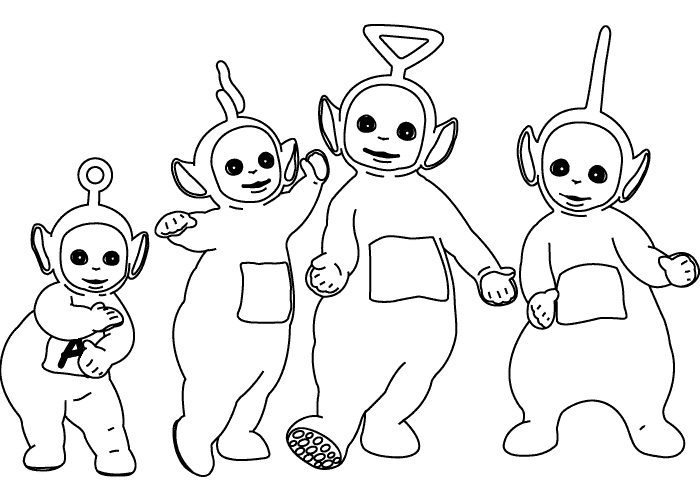
\includegraphics[width=\paperwidth,height=\paperheight]{a.png}};
\section{背景}
\subsection{tikz 實現}
編譯第一次會怪怪的,再一次就ok
\clearpage


\newpage



\AddToShipoutPictureBG*{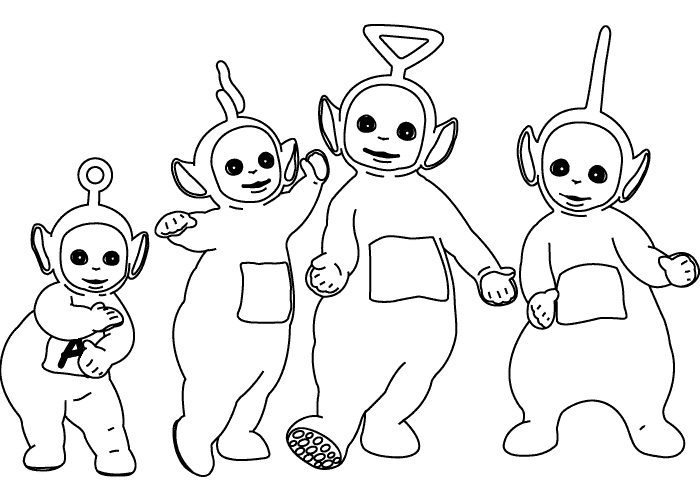
\includegraphics[width=\paperwidth,height=\paperheight]{a.png}}

\subsection{eso-pic}
text
\clearpage

\section{怪東西}
\subsection{對對齊}
\url{https://zhuanlan.zhihu.com/p/99406531}

\begin{table}[htb]
	\begin{tabular}{ccc}
		\toprule
		{ Joint} & {hi} & {hi} \\ \midrule
		{1} & {[\textover{0}{100}, 500]} & {[\textover[c]{1}{100}, 1000]} \\
		{2} & {[\textover[c]{0}{100}, 500]} & \textover[c]{1}{100}, \textover[c]{1000}{1111} \\
    3 & [\textover[r]{0}{100}, 500] & \textover[c]{1}{100}, \textover[c]{1000}{1111} \\
		\bottomrule
			\end{tabular}
\end{table}



\bibliography{bibfile} 
\bibliographystyle{unsrt}
